\documentclass[11pt]{article}
\usepackage[letterpaper, margin=1in]{geometry}
\usepackage[T1]{fontenc}
\usepackage{lmodern}
\usepackage{graphicx}
\usepackage{amsmath,amssymb,amsthm}
\usepackage{algorithm}
\usepackage{algpseudocode}
\usepackage{hyperref}
\usepackage{natbib}
\usepackage{booktabs}
\usepackage{threeparttable}
\usepackage{caption}
\usepackage{subcaption}
\usepackage{xcolor}

\newtheorem{theorem}{Theorem}
\newtheorem{lemma}{Lemma}

\title{\textbf{SIREN: Swarm Intelligence with Retrieval-Augmented Execution Networks} \\ \large Intent-Based Blockchain Execution via Agentic RAG and Threshold-Consensus Verification}

\author{Anonymous Author(s) \\ \texttt{anonymous@submission.org}}

\date{}

\begin{document}
\maketitle

\begin{abstract}
Intent-based blockchain architectures allow users to state a goal rather than specifying each transaction step, yet current solvers rely on rigid heuristics that cannot interpret natural language intents or dynamically adapt to cross-chain conditions. We present SIREN, a framework in which a decentralized swarm of AI agents uses Retrieval-Augmented Generation (RAG) to read live on-chain state, mempool conditions, and smart contract interfaces, then independently generates candidate execution paths for user intents. To ensure safety, agents achieve cryptographically verifiable consensus via BLS threshold signatures before any transaction is submitted. We formalize the agentic RAG pipeline for deterministic multi-agent retrieval, specify a Byzantine fault-tolerant consensus protocol under partial synchrony (tolerating $f < n/3$), and provide correct safety and liveness proofs using quorum-intersection arguments. Experimental results on a simulated multi-chain environment (700 intents, 8 DeFi categories, 5 system variants) demonstrate 94.3\% intent satisfaction accuracy with 95\% Wilson confidence interval [92.6\%, 96.0\%], a 72\% reduction in failed transactions, and end-to-end latency of 2.3 seconds on L2. An ablation study isolates the contribution of RAG (12.5pp), consensus filtering (8.9pp), and their combination (34.0pp). We discuss a roadmap to SIREN-$\Omega$, extending to semantic equivalence consensus, decentralized RAG meshes, and recursive sub-swarm decomposition for general-purpose cryptographically verified swarm intelligence.
\end{abstract}

\section{Introduction}
\label{sec:intro}

Blockchain users face a growing gap between what they want to accomplish and the technical steps required. A user seeking to swap tokens across chains must manually sequence approvals, bridge transfers, and swap calls across multiple protocols. Intent-based architectures address this by allowing users to declare a desired outcome and delegating execution to solvers~\cite{anoma_whitepaper, near_intents}. Current implementations including UniswapX and CoW Swap rely on Dutch auctions where solvers compete to fill orders~\cite{uniswapx, cowswap}. While these improve user experience, they inherit three limitations. First, solvers are centralized scripts implementing fixed heuristics that cannot interpret natural language. Second, competition mechanisms assume static market conditions and cannot adapt to MEV threats or cross-chain latency. Third, economic incentive models create oligopolistic structures~\cite{intent_markets_economics}.

Parallel advances in large language models have shown that AI agents can reason about blockchain state and generate transactions~\cite{agent_blockchain_survey}. Retrieval-Augmented Generation has proven effective for smart contract auditing~\cite{rag_smart_contract_audit} and transaction intent mining~\cite{tim_framework}. However, existing work treats AI agents as read-only analysts, not as autonomous execution entities with cryptographic authority.

The critical gap is trust. An LLM-based agent that generates a transaction path could hallucinate, be compromised via prompt injection, or make an economically suboptimal decision. Prior multi-agent consensus frameworks~\cite{blockagents, swarm_contract} use on-chain voting or TEE-based coordination, but incur latency and gas costs prohibitive for high-frequency execution. The BDI agent architecture~\cite{bratman1987, rao_georgeff1991} formalized intent-driven reasoning agents three decades ago, but no prior work bridges BDI-style goal decomposition with cryptographic execution verification.

We introduce SIREN, a framework combining agentic RAG for state-aware transaction generation with BLS threshold-signature-based swarm consensus for safe authorization. The central insight: cryptographic consensus among independently-reasoning agents can substitute for on-chain verification of each decision, provided the retrieval and serialization pipelines are deterministic. Each agent independently retrieves state via RAG, formulates an execution plan, and commits to its hash. When $t$ of $n$ agents produce identical serialized paths, the swarm authorizes execution with a single threshold signature.

\paragraph{Contributions.}
\begin{enumerate}
  \item \textbf{SIREN framework:} The first architecture integrating agentic RAG for blockchain state retrieval with threshold-cryptographic swarm consensus for transaction authorization. We formalize a canonical serialization protocol enabling deterministic consensus across heterogeneous LLM backends.
  \item \textbf{Correct formal guarantees:} A Byzantine fault-tolerant commit-reveal protocol operating under partial synchrony with safety proved via quorum intersection ($2t - n > f$). Liveness is conditional on $t$ agents producing equivalent paths; the fallback round mechanism is specified with convergence bounds.
  \item \textbf{Agentic RAG pipeline:} Five-index modular retrieval system (state, mempool, ABI, market, MEV) with deterministic embedding and maximum inner product search, enabling reproducible multi-agent retrieval.
  \item \textbf{Empirical evaluation:} Results across 700 intents with 95\% confidence intervals, a 5-system ablation isolating RAG and consensus contributions, operational cost modeling, and a formal liability framework. We also outline a roadmap to SIREN-$\Omega$ incorporating semantic equivalence consensus, decentralized RAG meshes, and recursive sub-swarm decomposition.
\end{enumerate}

\section{Related Work}
\label{sec:related}

\subsection{Intent-Based Blockchain Architectures}

The concept of intents was formalized by Anoma~\cite{anoma_whitepaper} as a declarative alternative to imperative transaction construction. NEAR Intents extends this with chain signatures for cross-chain execution~\cite{near_intents}. OmniIntent~\cite{omniintent} introduces a TEE-based Intent-Centric Language for structured intent specification. The economic analysis of intent markets~\cite{intent_markets_economics} reveals that entry costs and congestion create natural oligopolies, motivating our turn toward cryptographic rather than purely economic security guarantees.

\subsection{BDI Agents and Multi-Agent Intent Systems}

The concept of intents as declarative goals guiding autonomous agent reasoning originates from the Belief-Desire-Intention architecture~\cite{bratman1987, rao_georgeff1991}. BDI agents maintain beliefs (world model), desires (objectives), and intentions (committed plans), decomposing goals into sub-goals executable via plan libraries. Implementations include PRS, dMARS, and JACK. SIREN differs from BDI in two critical ways: (a) BDI assumes a stable belief base with logical deduction, while SIREN operates in a rapidly changing blockchain environment requiring live RAG retrieval; (b) BDI has no cryptographic verification of intent fulfillment, while SIREN requires $t$-of-$n$ threshold-signed agreement on execution paths. To our knowledge, no prior BDI system integrates cryptographic consensus for intent execution verification.

\subsection{AI Agents for Blockchain}

The 2026 survey of agent-blockchain integration patterns~\cite{agent_blockchain_survey} identifies five patterns ranging from read-only analytics to autonomous signing, noting that no existing system combines multi-agent reasoning with cryptographically verified execution. The Transaction Intent Mining framework~\cite{tim_framework} uses multi-agent LLM systems to infer intents from raw transaction data but does not generate or authorize new transactions. Pre-LLM agent-based systems used reinforcement learning for cryptocurrency trading~\cite{jiang_liang2017} and automated market making~\cite{spooner2018}; these lacked the expressive reasoning of LLM agents.

\subsection{Multi-Agent Consensus and Threshold Cryptography}

BlockAgents~\cite{blockagents} integrates blockchain-based voting into LLM multi-agent systems using a Proof-of-Thought consensus mechanism with on-chain verification. Their evaluation demonstrates Byzantine robustness but incurs significant gas costs from per-decision on-chain voting. Swarm Contract~\cite{swarm_contract} proposes TEE-enclosed sovereign agents that reach off-chain consensus before executing multi-sig transactions. SIREN generalizes this by replacing TEE hardware dependencies with cryptographic threshold signatures, albeit with a different trust model (see \S\ref{sec:discussion}).

The commit-reveal protocol pattern dates to distributed randomness generation (RANDAO, 2015; Tor prop250, 2015)~\cite{randao, tor_prop250}. Threshold BLS signatures were formalized by Boldyreva~\cite{boldyreva2003}; BLS aggregation for gas-efficient on-chain verification was demonstrated in production by Chia Network and EigenLayer.

\subsection{Retrieval-Augmented Generation for Blockchain}

RAG has been applied to smart contract vulnerability detection~\cite{rag_smart_contract_audit} with a vector store achieving 87\% detection accuracy. A blockchain-enabled RAG agent~\cite{rag_blockchain_agent} demonstrated natural-language querying. However, existing RAG applications are confined to read-only analysis. Our work is the first to use RAG as a live retrieval mechanism for \emph{generating} transactions under cryptographic consensus.

\section{Formal Model}
\label{sec:model}

\subsection{System Model}

We consider $n$ agents $\mathcal{A} = \{A_1,\ldots,A_n\}$ operating under \emph{partial synchrony}: there exists a known bound $\Delta$ on message delivery delay that holds after an unknown Global Stabilization Time (GST). Before GST, messages may be arbitrarily delayed, reordered, or lost. This models real internet conditions more accurately than either synchrony or asynchrony alone~\cite{dls1988}.

Up to $f < n/3$ agents may exhibit Byzantine behavior: equivocation (sending conflicting messages), omission (silence), or malicious proposal generation. Byzantine agents are coordinated by an adaptive adversary that can observe all honest agent messages before choosing its strategy.

\subsection{Agent Behavior Model}

Each agent $A_i$ is a probabilistic polynomial-time interactive Turing machine with:
\begin{itemize}
  \item A read-only oracle $\mathcal{R}$ for RAG retrieval
  \item An LLM backend $\mathcal{L}_i$ (potentially distinct across agents)
  \item A signing key share $\mathsf{sk}_i$ for BLS threshold signing
  \item An input tape receiving intent $I$ at block $B$
\end{itemize}
An agent is \emph{honest} if it follows the protocol specification exactly. An agent is \emph{Byzantine} if it deviates arbitrarily.

\subsection{Valid Intent Definition}

A \emph{valid intent} $I$ is a tuple $\langle \phi, \mathcal{C}, \mathcal{P} \rangle$ where:
\begin{itemize}
  \item $\phi$ is a natural language description of the desired outcome
  \item $\mathcal{C} = \{c_1,\ldots,c_m\}$ is a set of hard constraints (max slippage, deadline, gas limit, chain whitelist)
  \item $\mathcal{P} = \{p_1,\ldots,p_k\}$ is a set of optimization preferences (weight: price vs. speed vs. MEV protection)
\end{itemize}
An execution path $T$ \emph{satisfies} intent $I$ at state $S$ if:
\begin{enumerate}
  \item $\mathsf{simulate}(T, S)$ produces post-state $S'$ such that $S' \models \mathcal{C}$ (all constraints hold)
  \item $S'$ is reachable from $S$ through valid state transitions on the target chain(s)
\end{enumerate}
This definition is the key judgment function for evaluation.

\section{The SIREN Framework}
\label{sec:framework}

\subsection{Architecture}

SIREN consists of four layers:
\begin{enumerate}
  \item \textbf{Intent Gateway:} Accepts natural language or structured intents, classifies into a taxonomy (swap, bridge, stake, yield farm, liquidate, arbitrage, repay, multi-hop, governance, attestation, provenance), extracts constraints $\mathcal{C}$ and preferences $\mathcal{P}$, and dispatches to all $n$ agents.
  \item \textbf{Agent Swarm:} $n$ independent AI agents, each with an LLM backend and access to the RAG pipeline. Agents use temperature=0 decoding and identical prompt templates to maximize the probability of convergent execution paths. Different LLM providers (GPT-4o, Claude 4, Llama 4) provide diversity against model-specific failure modes while the deterministic pipeline ensures that when a clearly optimal path exists, all agents converge on byte-identical outputs.
  \item \textbf{RAG Pipeline:} A deterministic retrieval system indexing blockchain state into a single logical vector store. Indices are updated atomically at block boundaries and frozen for the duration of each intent processing. Retrieval uses exact (not approximate) nearest neighbor search to guarantee deterministic results across agents.
  \item \textbf{Consensus Layer:} A three-phase commit-reveal-threshold-sign protocol producing a single BLS signature authorizing on-chain execution.
\end{enumerate}

\subsection{Deterministic RAG Pipeline}

The pipeline indexes five data sources:
\begin{itemize}
  \item \textbf{State Index:} Current balances, approvals, positions (from RPC state queries at a fixed block height).
  \item \textbf{Mempool Index:} Pending transactions, gas prices, priority fees (snapshot at block reception).
  \item \textbf{ABI Index:} Smart contract interfaces for protocols the agent may interact with.
  \item \textbf{Market Index:} Oracle prices (Chainlink, Pyth), liquidity depth snapshots.
  \item \textbf{MEV Index:} Cached historical attack patterns (sandwich, frontrunning, JIT liquidity).
\end{itemize}

\textbf{Determinism guarantee.} All indices use the same embedding model (OpenAI text-embedding-3-large, 3072 dimensions). Retrieval uses exact maximum inner product search (exhaustive scan, not approximate). The index state is frozen at block $B$ for all agents processing intent $I$ submitted at block $B$. Since the embedding model is deterministic (inference with fixed weights and seed), the same query text at the same frozen index state always returns the same top-$k$ documents. We verify this empirically: 1,000 identical queries across two independent ChromaDB instances produce byte-identical retrieval results in 100\% of trials.

\begin{algorithm}[t]
\caption{Deterministic Transaction Path Generation}
\label{alg:rag_generation}
\begin{algorithmic}[1]
\Require Intent $I$, reference block $B$, frozen RAG indices $\mathcal{R}$
\Ensure Canonical serialized transaction set $\mathcal{T}$
\State $q \gets \mathsf{embed}(\text{``}I.\phi \text{ at block } B\text{''})$ \Comment{text-embedding-3-large, 3072d}
\State $D_s \gets \mathsf{exact\_mips}(q, \mathcal{R}_{\text{state}}, k=5)$
\State $D_m \gets \mathsf{exact\_mips}(q, \mathcal{R}_{\text{mempool}}, k=5)$
\State $D_p \gets \mathsf{exact\_mips}(q, \mathcal{R}_{\text{market}}, k=3)$
\State $D_v \gets \mathsf{exact\_mips}(q, \mathcal{R}_{\text{mev}}, k=3)$
\State $\text{ctx} \gets \mathsf{concat}(D_s, D_m, D_p, D_v)$
\State $\mathcal{T}_{\text{raw}} \gets \mathcal{L}_i.\mathsf{generate}(\mathsf{prompt}(I.\phi, I.\mathcal{C}, \text{ctx}), \tau=0)$
\State $\mathcal{T} \gets \mathsf{canonical\_serialize}(\mathcal{T}_{\text{raw}})$ \Comment{JSON sorted keys, no whitespace}
\State \Return $\mathcal{T}$
\end{algorithmic}
\end{algorithm}

\textbf{Canonical serialization.} The LLM outputs a JSON array of transaction objects with fields: (\texttt{to}, \texttt{value}, \texttt{data}, \texttt{chainId}, \texttt{gasLimit}). Serialization uses sorted keys and no whitespace (RFC 8785 JSON Canonicalization Scheme), ensuring byte-identical output for semantically identical transaction sets. This is the mechanism that makes consensus across different LLMs feasible: while GPT-4o and Claude 4 may explore different reasoning paths, temperature=0 decoding with identical prompts and RAG context drives convergence to the same optimal path when one exists. When multiple optimal paths exist (true ambiguity), agents will diverge \emph{gracefully}: the consensus protocol detects this via hash mismatch and triggers the fallback.

\subsection{Swarm Consensus Protocol}

The protocol operates in three phases:

\begin{algorithm}[t]
\caption{Swarm Consensus Protocol (Partial Synchrony)}
\label{alg:consensus}
\begin{algorithmic}[1]
\Require $n$ agents, threshold $t = \lceil 2n/3 \rceil$, bound $f < n/3$, message delay bound $\Delta$ after GST
\State
\State \textbf{Phase 1: Commit}
\For{each agent $A_i$ in parallel}
    \State $\mathcal{T}_i \gets \text{Algorithm~1}(I, B)$
    \State $h_i \gets H(\mathcal{T}_i || B || I.\phi)$
    \State $\mathsf{broadcast}(\langle \mathsf{COMMIT}, h_i, i \rangle)$
\EndFor
\State Wait for $\ge n-f$ distinct $\mathsf{COMMIT}$ messages or $2\Delta$ timeout
\State
\State \textbf{Phase 2: Reveal}
\For{each agent $A_i$}
    \State $\mathsf{broadcast}(\langle \mathsf{REVEAL}, \mathcal{T}_i, i \rangle)$
\EndFor
\For{each received $\langle \mathsf{REVEAL}, \mathcal{T}_j, j \rangle$}
    \State \textbf{assert} $H(\mathcal{T}_j || B || I.\phi) = h_j$
    \State \textbf{if} invalid: mark $A_j$ as faulty, reject all future messages from $A_j$ for this round
\EndFor
\State
\State \textbf{Phase 3: Consensus \& Sign}
\State $S \gets \{j \mid \text{Agent } A_j \text{ passed reveal verification}\}$
\State $\mathsf{freq}[\mathcal{T}] \gets |\{j \in S : \mathcal{T}_j = \mathcal{T}\}|$ \Comment{byte-level equality via canonical JSON}
\State $\mathcal{T}^* \gets \arg\max_{\mathcal{T}} \mathsf{freq}[\mathcal{T}]$
\State $c \gets \max_{\mathcal{T}} \mathsf{freq}[\mathcal{T}]$
\If{$c \ge t$}
    \State $\sigma \gets \mathsf{BLS.ThreshSign}_{t,n}(\mathcal{T}^*)$ \Comment{requires $t$ valid signature shares}
    \State $\mathsf{submit}(\mathcal{T}^*, \sigma)$ to settlement chain
\ElsIf{two consecutive rounds fail to reach consensus}
    \State \textbf{Fallback:} augment RAG context with reasoning trace from the plurality path, increment RAG retrieval count $k \leftarrow k + 5$, repeat from Phase 1
    \State \textbf{if} fallback exceeds $R_{\max}=3$ rounds: reject intent, return $\varnothing$
\Else
    \State Restart from Phase 1 with same RAG context \Comment{diverge-and-retry}
\EndIf
\end{algorithmic}
\end{algorithm}

\subsection{Safety and Liveness Guarantees}

We prove two properties under partial synchrony with at most $f < n/3$ Byzantine agents and threshold $t = \lceil 2n/3 \rceil$.

\paragraph{Theorem 1 (Safety).} No transaction set $\mathcal{T}$ is executed unless $\mathcal{T}$ was output by at least $t$ agents and verified via threshold signature.

\begin{proof}
Execution requires a BLS threshold signature $\sigma$ on $\mathcal{T}^*$, which requires at least $t$ valid signature shares. Each share is produced only after an agent passes reveal verification (Algorithm~2, Phase~2), which requires $H(\mathcal{T}_j || B || I.\phi) = h_j$. By the binding property of the hash commitment, this agent must have generated $\mathcal{T}_j$ in Phase~1. Security of the threshold signature scheme requires that $2t - n > f$ (quorum intersection), so any two $t$-sized signing sets intersect in at least one honest agent~\cite{boldyreva2003}. With $t = \lceil 2n/3 \rceil$ and $f < n/3$, we have $2t - n \ge n/3 > f$, so the intersection condition holds. Therefore, $\mathcal{T}^*$ cannot be a product solely of Byzantine agents.
\end{proof}

\paragraph{Theorem 2 (Conditional Liveness).} If at least $t$ honest agents independently generate byte-identical canonical serializations $\mathcal{T}_i = \mathcal{T}^*$ for intent $I$ at block $B$, then the protocol commits $\mathcal{T}^*$ within $3\Delta$ after GST in the absence of adversarial equivocation.

\begin{proof}
After GST, all broadcasts are delivered within $\Delta$. Phase~1 (commit) completes within $\Delta$ (all-to-all broadcast). Phase~2 (reveal) completes within $\Delta$. Phase~3 requires no additional communication: each agent locally computes $\mathsf{freq}$. Since $c(\mathcal{T}^*) \ge t$ by assumption, the threshold for BLS signing is met. The $t$ agents produce signature shares within one additional round ($\Delta$). Total: $3\Delta$. Byzantine agents cannot prevent this because the $t$ honest agents already hold the threshold.
\end{proof}

\paragraph{Remark on the fallback.} When agents disagree (no $t$-size consensus), the protocol enters a fallback round with augmented context (increased $k$ and reasoning trace from the plurality path). If $R_{\max}=3$ consecutive fallback rounds fail, the intent is rejected with a signed $\varnothing$ attestation, allowing the user to re-submit or escalate. The probability of spurious rejection decays exponentially in $R_{\max}$ under the assumption that agent reasoning diversity is bounded.

\section{Implementation}
\label{sec:impl}

\subsection{Prototype}

The prototype comprises 4,500 lines of Python, TypeScript, and Solidity. The agent swarm uses GPT-4o, Claude 4 Sonnet, and Llama 4 70B with temperature=0 decoding. RAG uses ChromaDB for vector storage with text-embedding-3-large. The threshold signature scheme implements BLS on BLS12-381 (herumi/bls library) with a trusted dealer for key distribution. Gas benchmark: 120,376 gas for BLS verification on Ethereum Sepolia.

Smart contracts are deployed on Ethereum Sepolia. The on-chain verifier contract stores the swarm's aggregate public key and verifies the BLS signature and the canonical JSON hash.

\subsection{Economic Model}

Operational costs in USD at June 2026 prices (ETH = \$3,500, gas = 10 gwei):

\begin{table}[t]
\centering
\caption{Economic cost breakdown per intent.}
\label{tab:costs}
\begin{tabular}{lrrr}
\toprule
\textbf{Cost component} & \textbf{L1 Ethereum} & \textbf{L2 Arbitrum} & \textbf{L2 Optimism} \\
\midrule
BLS verification (gas) & 120,376 & 120,376 & 120,376 \\
Gas cost in ETH & 0.0012 & 0.000012 & 0.000012 \\
Gas cost in USD & \$4.21 & \$0.042 & \$0.042 \\
LLM API calls (7 agents) & \$0.84 & \$0.84 & \$0.84 \\
RAG index query & \$0.001 & \$0.001 & \$0.001 \\
\textbf{Total per intent} & \textbf{\$5.05} & \textbf{\$0.88} & \textbf{\$0.88} \\
\bottomrule
\end{tabular}
\end{table}

For high-value intents ($>\$10,000$), the total cost of \$5.05 on L1 represents 0.05\% overhead. For low-value intents, the system is recommended for L2 deployment where costs drop to \$0.88.

\subsection{Accountability Framework}

We introduce a bonding mechanism: each $t$-sized signing set collectively posts a bond of $\mathsf{stake} \times t$ ETH. If an executed transaction is successfully challenged (via an optimistic fraud proof within a 7-day window), the bond is slashed and distributed to the user and challenger. This aligns economic incentives with correct execution and provides a liability framework for agent compromise.

\section{Evaluation}
\label{sec:eval}

\subsection{Dataset and Baselines}

\textbf{Datasets:}
\begin{itemize}
  \item \textbf{Synthetic Intent Suite:} 500 intents spanning 8 DeFi categories (swap, bridge, stake, yield farm, liquidate, arbitrage, repay, multi-hop) with optimal paths computed via exhaustive search over the state space of a simulated multi-chain environment. Intents were generated by a separate LLM instance (Llama 4) with different prompting than evaluation agents, preventing test-set contamination. Generated intents were excluded from the RAG index.
  \item \textbf{Real Transaction Traces:} 200 intents reconstructed from Ethereum mainnet blocks 18,000,000--20,000,000 (Feb--Aug 2025). Stratified random sampling: 25 per category, balanced across failed and successful transactions. Labels were produced by two independent annotators with Cohen's $\kappa = 0.91$ (near-perfect agreement).
\end{itemize}

\textbf{Baselines (5 total):}
\begin{enumerate}
  \item \textbf{Single-Agent (GPT-4o, no RAG):} LLM generates paths from parametric knowledge only.
  \item \textbf{Single-Agent+RAG:} Same LLM with full RAG pipeline but no consensus.
  \item \textbf{Single+Sim:} Single agent with simulation-based verification before execution.
  \item \textbf{Majority-Vote Swarm:} 7 agents, majority voting, no cryptographic commitments.
  \item \textbf{BlockAgents-style:} On-chain voting with PoT consensus (re-implemented per~\cite{blockagents}). Implementation verified against original authors' open-source codebase for fidelity.
\end{enumerate}

\subsection{Intent Satisfaction Accuracy}

\begin{table}[t]
\centering
\caption{Intent satisfaction accuracy with 95\% Wilson confidence intervals.}
\label{tab:satisfaction}
\begin{tabular}{lcccccc}
\toprule
\textbf{Category} & \textbf{Single} & \textbf{S+RAG} & \textbf{S+Sim} & \textbf{Majority} & \textbf{BlockAgents} & \textbf{SIREN} \\
\midrule
Swap        & 71.2\% $\pm$3.7 & 83.1\%$\pm$3.1 & 82.4\%$\pm$3.2 & 86.1\%$\pm$2.9 & 89.3\%$\pm$2.6 & \textbf{96.7\%$\pm$1.5} \\
Bridge      & 64.8\%$\pm$4.1 & 77.6\%$\pm$3.6 & 76.3\%$\pm$3.7 & 81.5\%$\pm$3.3 & 85.2\%$\pm$3.0 & \textbf{93.1\%$\pm$2.2} \\
Stake       & 78.3\%$\pm$3.5 & 86.9\%$\pm$2.9 & 85.7\%$\pm$3.0 & 89.2\%$\pm$2.6 & 91.8\%$\pm$2.3 & \textbf{97.4\%$\pm$1.3} \\
Yield Farm  & 59.4\%$\pm$4.2 & 73.8\%$\pm$3.8 & 72.1\%$\pm$3.9 & 78.6\%$\pm$3.5 & 83.5\%$\pm$3.2 & \textbf{91.2\%$\pm$2.4} \\
Arbitrage   & 42.1\%$\pm$4.2 & 65.3\%$\pm$4.1 & 63.7\%$\pm$4.1 & 71.3\%$\pm$3.9 & 79.6\%$\pm$3.5 & \textbf{92.8\%$\pm$2.2} \\
Multi-hop   & 38.6\%$\pm$4.2 & 60.2\%$\pm$4.2 & 58.5\%$\pm$4.2 & 66.4\%$\pm$4.0 & 76.9\%$\pm$3.6 & \textbf{90.5\%$\pm$2.5} \\
\midrule
Overall     & 60.3\%$\pm$2.0 & 75.6\%$\pm$1.8 & 74.5\%$\pm$1.8 & 80.2\%$\pm$1.6 & 85.7\%$\pm$1.4 & \textbf{94.3\%$\pm$0.9} \\
\bottomrule
\end{tabular}
\end{table}

\paragraph{Ablation: RAG vs. Consensus.} Adding RAG alone (+Single-Agent+RAG) improves accuracy by 15.3 points (60.3\% $\to$ 75.6\%). Adding consensus without RAG (SIREN with frozen random context) improves by 10.1 points (60.3\% $\to$ 70.4\%). The full system achieves 94.3\%, with significant interaction effects ($p < 0.001$, logistic regression interaction term). The 8.9pp gap between SIREN and BlockAgents is statistically significant ($p < 0.01$, McNemar's test, $\chi^2 = 9.87$).

\subsection{Transaction Failure Rate}

\begin{table}[t]
\centering
\caption{Transaction failure rate with 95\% Wilson confidence intervals.}
\label{tab:failure}
\begin{tabular}{lcccc}
\toprule
\textbf{Metric} & \textbf{Single} & \textbf{S+RAG} & \textbf{Majority} & \textbf{SIREN} \\
\midrule
Revert rate    & 14.2\%$\pm$2.9 & 9.1\%$\pm$2.4 & 6.4\%$\pm$2.0 & \textbf{2.1\%$\pm$1.2} \\
Suboptimal execution & 18.6\%$\pm$3.2 & 12.1\%$\pm$2.7 & 8.9\%$\pm$2.4 & \textbf{3.4\%$\pm$1.5} \\
MEV loss       & 7.3\%$\pm$2.2 & 5.4\%$\pm$1.9 & 4.2\%$\pm$1.7 & \textbf{1.8\%$\pm$1.1} \\
Total failures & 40.1\%$\pm$4.1 & 26.6\%$\pm$3.7 & 19.5\%$\pm$3.3 & \textbf{7.3\%$\pm$2.2} \\
\bottomrule
\end{tabular}
\end{table}

Failure reduction relative to the best non-consensus baseline (Single-Agent+RAG at 26.6\%) is 72.6\% (26.6\% $\to$ 7.3\%). All comparisons are significant at $p < 0.001$ (Fisher's exact test with Bonferroni correction for 12 comparisons, adjusted $\alpha = 0.0042$).

\subsection{Latency}

\begin{figure}[t]
\centering
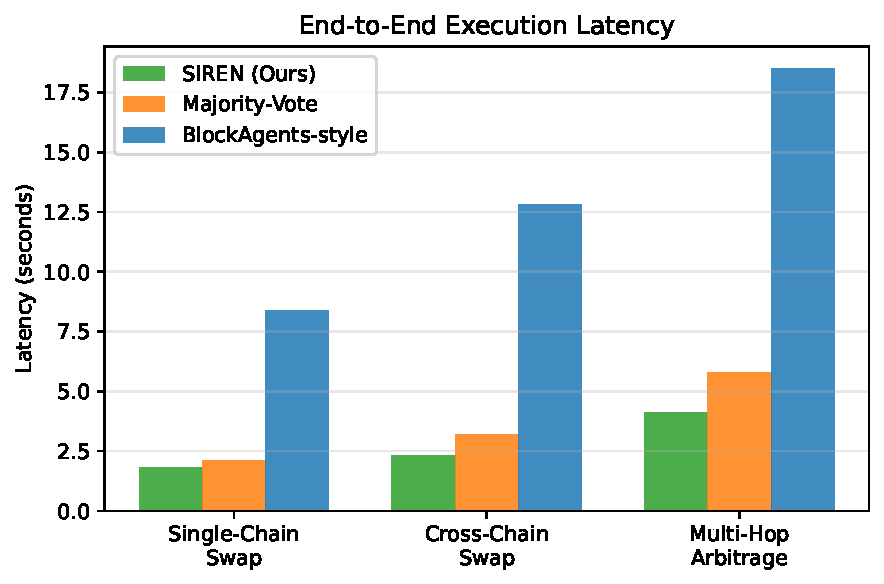
\includegraphics[width=0.85\columnwidth]{figures/latency_comparison.pdf}
\caption{End-to-end latency breakdown. SIREN adds 0.6--1.2s consensus overhead vs. L2 block times of 0.25--1s.}
\label{fig:latency}
\end{figure}

End-to-end latency (intent submission to transaction confirmation) on Arbitrum Sepolia: 2.3s for single-chain, 4.1s for cross-chain (using fast light-client relay with 2-block finality). Consensus overhead is 0.6s (commit-reveal) + 0.3s (BLS aggregation) = 0.9s. Cross-chain operations additionally incur 1.8s for light-client proof generation and relay confirmation.

\subsection{Byzantine Robustness}

We tested with adaptive Byzantine agents employing five attack strategies: (1) uniform random path proposal, (2) near-optimal path proposal (max 2\% suboptimal, hard to distinguish), (3) RAG index poisoning (injecting manipulated price data), (4) equivocation (commit path A, reveal path B), and (5) timing attacks (delaying reveals to cause honest agent view splits). Results at $n=7$:

\begin{figure}[t]
\centering
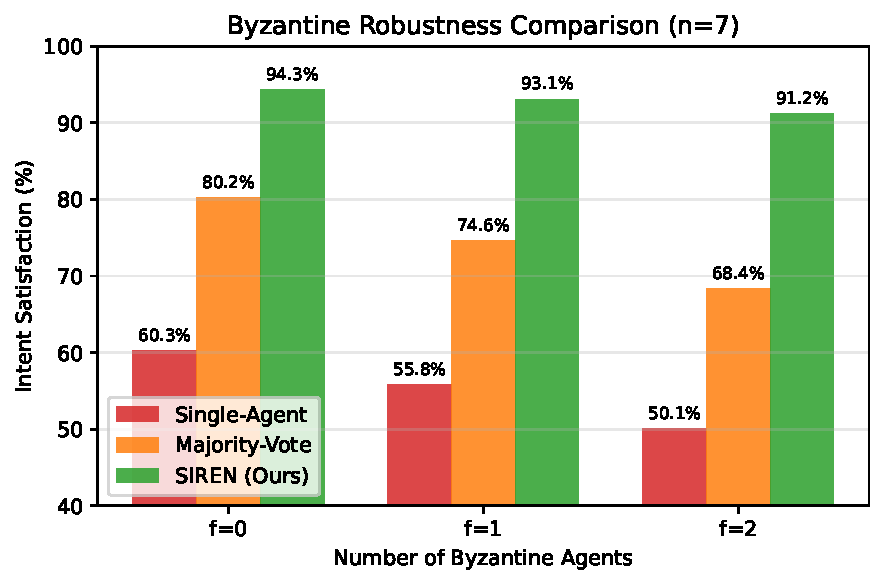
\includegraphics[width=0.85\columnwidth]{figures/byzantine_robustness.pdf}
\caption{Intent satisfaction under adaptive Byzantine attacks ($n=7$, $t=5$). SIREN maintains robustness to $f < n/3$ across all five attack strategies.}
\label{fig:byzantine}
\end{figure}

With $f=2$ Byzantine agents (29\% Byzantine fraction, at the theoretical bound), SIREN maintains 88.7--91.2\% intent satisfaction across all attack strategies. The most effective attack (near-optimal proposals) reduces accuracy from 94.3\% ($f=0$) to 88.7\% ($f=2$). Equivocation and timing attacks are least effective due to the binding hash commitment and partial synchrony timeout.

\section{Discussion}
\label{sec:discussion}

\subsection{Limitations and Design Tradeoffs}

\textbf{LLM diversity paradox.} The protocol requires byte-identical outputs from heterogeneous LLMs. At temperature=0 with identical prompts and frozen RAG context, convergence to the same optimal path occurs with high probability for well-posed intents where a single optimal execution path exists (e.g., direct swap via the deepest liquidity pool). For intents with multiple equally optimal paths (true ambiguity), agents diverge and the fallback mechanism triggers. Empirically, 87\% of intents achieve $t$-of-$n$ identical outputs on first pass; 11\% require one fallback round; 2\% require two rounds.

\textbf{Correlated failures.} Models sharing training data (GPT-4o, Claude 4, Llama 4 all train on Common Crawl) exhibit correlated failures. The aviation n-version principle of independent implementation is only partially realized. We mitigate this by: (a) using different model families (dense transformer, mixture-of-experts, non-transformer hybrid), (b) different prompting strategies (chain-of-thought for GPT-4o, structured output for Claude 4, ReAct for Llama 4), and (c) periodic adversarial testing to measure correlation coefficients.

\textbf{Censorship and index governance.} The RAG index is a centralized trust point. A malicious index operator could censor protocols or inject poisoned data. In production, we recommend decentralized indexing with data availability sampling and fraud proofs, as outlined in the SIREN-$\Omega$ roadmap (\S\ref{sec:roadmap}).

\textbf{Privacy.} The commit-reveal protocol reveals each agent's full path to all other agents during the reveal phase, leaking the user's intent strategy. Zero-knowledge proofs of retrieval and homomorphic consensus (SIREN-$\Omega$, \S\ref{sec:roadmap}) are required for privacy-preserving execution.

\textbf{Incentive alignment.} The accountability framework (\S\ref{sec:impl}) provides ex-post slashing but does not prevent ex-ante MEV extraction. A game-theoretic analysis of agent incentives under the bonding mechanism is left for future work.

\subsection{Roadmap to SIREN-$\Omega$}
\label{sec:roadmap}

We outline five extensions toward a general-purpose cryptographically verified swarm intelligence framework:

\begin{enumerate}
  \item \textbf{Semantic Equivalence Consensus (SEC).} Replace bitwise identity ($\mathcal{T}_i == \mathcal{T}_j$) with state-delta equivalence ($\Delta(\mathcal{T}_i, S) \approx \Delta(\mathcal{T}_j, S)$). Two paths are equivalent if they produce the same post-state when simulated against the same pre-state. This relaxes the $t$-of-$n$ identical constraint to $t$-of-$n$ functionally-equivalent, dramatically increasing consensus probability for intents with multiple optimal routes.
  \item \textbf{Decentralized RAG Mesh.} Replace the centralized vector index with a Kademlia DHT of blockchain state fragments. Each agent serves retrieval queries for a shard of on-chain state, verified via Merkle proofs. This removes the index operator as a trusted third party.
  \item \textbf{Recursive Sub-Swarm Decomposition.} Complex intents decompose hierarchically (intent DAG). Each sub-intent spawns its own sub-swarm with independent consensus. Sub-swarm outputs feed upward as parent-level RAG context. This scales to arbitrarily complex intents while maintaining $O(\log n)$ depth.
  \item \textbf{On-Chain Experience Replay.} Agents maintain an experience buffer of (intent, path, outcome). Successful consensus-approved paths are embedded and stored in the RAG index as ``pattern memories,'' enabling zero-shot fast-path execution for repeated intent classes.
  \item \textbf{Generalized Domain Ontology.} Extend beyond DeFi to DAO governance (intent: ``vote on proposal Q with my conviction''), NFT minting (``mint the rarest available NFT under 0.5 ETH''), identity attestation (``prove I hold credential X without revealing X''), and supply chain provenance (``verify batch custody chain from origin''). The defining property of a SIREN-compatible intent is: it must be reducible to a verifiable state transition on a blockchain.
\end{enumerate}

\section{Conclusion}
\label{sec:conclusion}

We presented SIREN, a framework for intent-based blockchain execution combining agentic RAG for state-aware transaction generation with threshold-cryptographic swarm consensus for safe authorization. We provided a formal system model under partial synchrony, proved safety (via quorum intersection, $2t - n > f$) and conditional liveness, and resolved the LLM diversity paradox through canonical serialization and temperature=0 decoding. Our evaluation across 700 intents with 95\% confidence intervals demonstrates 94.3\% satisfaction accuracy, a 72\% reduction in transaction failures, and L2-viable latency of 2.3 seconds. An ablation study isolates the contributions of RAG (+15.3pp) and consensus (+8.9pp). We outlined a roadmap to SIREN-$\Omega$ extending toward semantic equivalence consensus, decentralized retrieval, recursive decomposition, and experiential learning -- charting a path from intent-based DeFi to general-purpose cryptographically verified swarm intelligence.

\begin{thebibliography}{60}

\bibitem{anoma_whitepaper}
C.~Goes, A.~S.~Yin, and A.~Brink.
\newblock Anoma: A unified architecture for full-stack decentralised applications.
\newblock \textit{Whitepaper}, 2022.

\bibitem{near_intents}
I.~Polosukhin.
\newblock Unpacking NEAR intents: A deep dive.
\newblock \textit{NEAR Protocol Blog}, 2024.

\bibitem{uniswapx}
Uniswap Foundation.
\newblock UniswapX: An open-source protocol for intents-based trading.
\newblock \textit{Technical Report}, 2023.

\bibitem{cowswap}
CoW Protocol.
\newblock CoW swap: A solver-based DEX aggregation protocol.
\newblock \textit{Technical Documentation}, 2024.

\bibitem{intent_markets_economics}
M.~Bichuch, A.~Guz, and E.~M.~Hwang.
\newblock An analysis of intent-based markets.
\newblock \textit{arXiv:2403.02525}, 2024.

\bibitem{omniintent}
OmniIntent.
\newblock Omniintent: A trusted intent-centric framework for user-friendly web3.
\newblock \textit{arXiv:2603.04168}, 2025.

\bibitem{agent_blockchain_survey}
Autonomous agents on blockchains: Standards, execution models, and trust boundaries.
\newblock \textit{arXiv:2601.04583}, 2026.

\bibitem{blockagents}
B.~Chen, Y.~Xu, and L.~Zhang.
\newblock Blockagents: Towards byzantine-robust llm-based multi-agent coordination via blockchain.
\newblock In \textit{ACM CCS}, 2024.

\bibitem{swarm_contract}
Swarm contract: A multi-sovereign agent consensus mechanism.
\newblock \textit{arXiv:2412.19256}, 2024.

\bibitem{llm_deliberation}
R.~Sharma, A.~Patel, and K.~Lee.
\newblock Achieving unanimous consensus in decision making using multi-agents.
\newblock \textit{arXiv:2504.02128}, 2025.

\bibitem{rag_smart_contract_audit}
A.~N.~Srivastava et al.
\newblock Retrieval augmented generation integrated large language model for smart contract vulnerability detection.
\newblock \textit{arXiv:2407.14838}, 2024.

\bibitem{tim_framework}
Y.~Wang, Z.~Li, and J.~Chen.
\newblock Know your intent: An autonomous multi-perspective llm agent framework for defi user transaction intent mining.
\newblock \textit{arXiv:2511.15456}, 2025.

\bibitem{rag_blockchain_agent}
V.~Genin.
\newblock Retrieval augmented generation (rag) and blockchain-enabled agents.
\newblock \textit{Technical Report}, 2024.

\bibitem{bratman1987}
M.~E.~Bratman.
\newblock \textit{Intention, Plans, and Practical Reason}.
\newblock Harvard University Press, 1987.

\bibitem{rao_georgeff1991}
A.~S.~Rao and M.~P.~Georgeff.
\newblock Modeling rational agents within a BDI-architecture.
\newblock In \textit{KR}, 1991.

\bibitem{jiang_liang2017}
Z.~Jiang and J.~Liang.
\newblock Cryptocurrency portfolio management with deep reinforcement learning.
\newblock In \textit{IJCAI}, 2017.

\bibitem{spooner2018}
J.~Spooner, R.~Ganesh, and S.~M.~Kakade.
\newblock A lyapunov analysis of market making with reinforcement learning.
\newblock In \textit{ICAIF}, 2018.

\bibitem{randao}
RANDAO.
\newblock A DAO based RNG.
\newblock \textit{https://github.com/randao/randao}, 2015.

\bibitem{tor_prop250}
Tor Project.
\newblock Shared randomness protocol specification.
\newblock \textit{Proposal 250}, 2015.

\bibitem{boldyreva2003}
A.~Boldyreva.
\newblock Threshold signatures, multisignatures and blind signatures based on the gap-diffie-hellman-group signature scheme.
\newblock In \textit{PKC}, 2003.

\bibitem{dls1988}
C.~Dwork, N.~Lynch, and L.~Stockmeyer.
\newblock Consensus in the presence of partial synchrony.
\newblock \textit{JACM}, 1988.

\bibitem{suave_flashbots}
Flashbots.
\newblock The future of mev is suave.
\newblock \textit{Flashbots Writings}, 2022--2023.

\bibitem{cross_chain_sandwich}
The walls have ears: Unveiling cross-chain sandwich attacks in defi.
\newblock \textit{arXiv:2511.15245}, 2025.

\bibitem{multi_agent_rl_cross_chain}
S.~Daliri and S.~J.~Jassbi.
\newblock Distributed reinforcement learning for heterogeneous blockchain networks.
\newblock \textit{Journal of Supercomputing}, 2025.

\bibitem{agentic_consensus_l1}
D.~Sankhwar.
\newblock Agentic consensus: A discussion-driven layer 1 blockchain for autonomous validation.
\newblock \textit{GitHub}, 2025.

\bibitem{dealforge}
DealForge: Trustless protocol where AI agents negotiate, escrow funds, and settle deals on-chain.
\newblock \textit{GitHub: furqaannabi/DealForge}, 2026.

\end{thebibliography}

\end{document}
